% https://www.irasutoya.com/2019/04/blog-post_87.html
\begin{frame}{Hank}
	\centering

	\note<1->[item]{Hank neuer Mitarbeiter bei AC-Games}

	\note<2->[item]{Ist Datenbankadmin}
	\note<2->[item]{Hat nicht vor lange bei der Firma zu bleiben}
	\note<2->[item]{Hat Walters alten Blogpost gelesen}

	\note<3->[item]{Ist auch verwundert über hohen Preis}
	\note<3->[item]{Will schauen was aus den Daten rauszuholen ist}


	\begin{tikzpicture}
		\node<1-2> (hank) {
\includegraphics[height=0.15\textwidth]{images/hank}};
		\node[below =0cm of hank] (hank-name) {Hank};

		% Pack Server hin

		\node<2->[right =4cm of hank] (server) {
\includegraphics[height=0.15\textwidth]{images/server}};
		\node<2->[below =0cm of server] (server-name) {Datenbank};

		\draw<2->[-stealth] (hank) -- node[above] {Admin} (server);

		% "Mal rumprobieren"
		\node<3-> (hank) {
\includegraphics[height=0.15\textwidth]{images/hank_hmm}};
		\node<3->[above right=-8mm and 0mm of hank] (speech) {\includesvg[width=0.25\textwidth]{images/thought_bubble}};
		\node<3->[above right = -3mm and -1mm of speech.center, label={[align=center]Mal schauen}] (wenig-daten) {};
	\end{tikzpicture}
\end{frame}

\begin{frame}{Das Experiment}
	\centering

	\note<1-4>[item]{Berechnungen auf dem Daten}
	\note<2-4>[item]{Nutzer lassen sich nach Verhalten in Kategorien einteilen}
	\note<3-4>[item]{Stress-Typen}
	\note<4>[item]{Neugier-Typen}
	\note<4>[item]{Nicht wirklich beschrieben, was diese ausmacht \begin{itemize}
			\item Auch nicht so wichtig
		\end{itemize}}
	\note<5->{Im In-Game Shop \begin{itemize}
			\item Programmiert künstlichen Zähler (\#Vorrätige Exemplare)
			\item Auf Nutzer-Typ angepasst
			\item Für Stress-Typen \begin{itemize}
				      \item Anfangs 2-stellige Zahl
				      \item Tickt langsam runter
			      \end{itemize}
			\item Für Neugier-Typen \begin{itemize}
				      \item Zeigt zuerst keine Zahl sondern \enquote{Vorrat prüfen} Knopf
				      \item Dann wird \enquote{Nur noch 1 Exemplar} angezeigt
			      \end{itemize}
		\end{itemize}}

	\visible<2->{\begin{tabular}{c|lll}
			\textbf{Typ} & \textbf{Nutzer:innen}                                  \\\hline \hline\onslide<3->
			Stress       & Bob L.                & Lina M.  & \dots  \onslide<4-> \\\hline
			Neugier      & Katie A.              & Chris O. & \dots               \\
			\vdots       & \dots                 &          &
		\end{tabular}}
\end{frame}

\begin{frame}{Die Ergebnisse}
	\centering

	\note<1->{Nächster Abend: Hank prüft die Verkaufszahlen}
	\note<2->{Umgestaltung des Shop hat Kaufverhalten stark beeinflusst}
	\note<3->{Fragt sich: Was kann noch alles mit den Daten angestellt werden. \begin{itemize}
			\item mit Kunden von AC-Games
			\item vielleicht auch außerhalb?
		\end{itemize}}

	\begin{tikzpicture}
		\node<1> (hank) {
\includegraphics[width=0.15\textwidth]{images/hank}};
		\node[below =0cm of hank] (hank-name) {Hank};

		\node<2> (hank) {
\includegraphics[width=0.15\textwidth]{images/hank_surprise}};
		\node<2>[right =2cm of hank] (more_money) {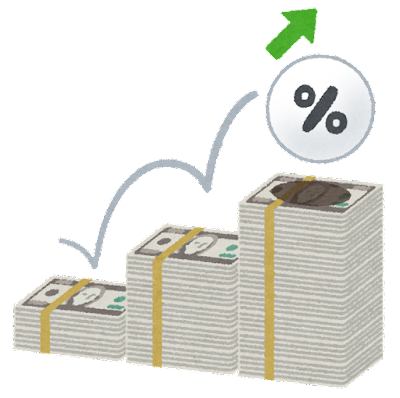
\includegraphics[width=0.2\textwidth]{images/more_money}};

		\node<3> (hank) {
\includegraphics[width=0.15\textwidth]{images/hank_worried}};
		\node<3->[above right=-8mm and -2mm of hank] (speech) {\includesvg[width=0.25\textwidth]{images/thought_bubble}};
		\node<3->[above right = -5mm and -1mm of speech.center, label={[align=center]Damit kann man\\echt Mist bauen...}] (wenig-daten) {};
	\end{tikzpicture}
\end{frame}

